\section{Proposta para Melhoria na Aquisição da Nuvem de Pontos} \label{pontosProposta}

Além do uso de imagens HDR tonemapped, outra proposta deste trabalho para melhorar a qualidade e quantidade de elementos da nuvem de pontos gerada se baseia no processamento de realce de contornos dessas imagens. A hipótese é que com contornos mais acentuados os algoritmos de identificação de pontos de interesse identificarão mais pontos e gerarão nuvens com maior qualidade.

Para isso foi proposto o uso do filtro de Laplace, que se trata de um método conhecido em processamento de imagens para realce de contornos. Este método se baseia no conceito da soma das derivadas parciais de segunda ordem \cite{gonzalez} para realçar os contornos da imagem. A Equação \ref{eqPontosLaplace} mostra operador de Laplace: \cite{gonzalez}

\begin{align} \label{eqPontosLaplace}
	\nabla f^2 = \frac{\partial^2f}{\partial x^2} + \frac{\partial^2f}{\partial y^2}
\end{align}

Para o processamento digital de imagens essa equação é transformada para a sua forma discreta como mostrado na Equação \ref{eqPontosLaplaceDisc}. \cite{gonzalez}

\begin{align} \label{eqPontosLaplaceDisc}
	\nabla f^2 = -4f(x,y) + f(x+1,y) + f(x-1,y) + f(x,y+1) + f(x,y-1)
\end{align}

Segundo Gonzalez \cite{gonzalez}, a Equação \ref{eqPontosLaplaceDisc} resulta numa máscara que leva em consideração as variações de cores dos pixels vizinhos que formam ângulos múltiplos de $90º$ em relação ao pixel central. Gonzalez \cite{gonzalez} ainda acrescenta que as diagonais podem ser adicionadas à máscara resultando na matriz mostrada na Figura \ref{figPontosLaplaceMat}.

\begin{figure}[H]
  \centering
  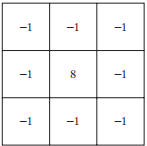
\includegraphics[height=3cm]{matrizLaplace}
  \caption{Filtro de Laplace.}
  \label{figPontosLaplaceMat}
\end{figure}

Uma vez com os contornos da imagem sendo extraídos com o filtro de Laplace, é feita a soma da imagem inicial com estes para que seja obtido o realce dos contornos da imagem. Neste processo será utilizado um fator $\alpha$, $0 < \alpha < 1$, para regular a intensidade de realce das bordas. A Equação \ref{eqPontosLaplaceSoma} ilustra o processo de realce das bordas.

\begin{align} \label{eqPontosLaplaceSoma}
	Imagem_{final} = Imagem_{inicial} + \alpha f(Imagem_{inicial})
\end{align}
Onde
\begin{itemize}
\item $f$ é o filtro de Laplace.
\end{itemize}

  Sendo assim, o processo geral proposto para obtenção da nuvem de pontos a partir de imagens HDR segue as seguintes etapas:

\begin{enumerate}
\item Geração das imagens HDR a partir de conjuntos de imagens LDR.
\item \textit{Tone mapping} das imagens HDR geradas.
\item Realce das bordas das imagens \textit{tonemapped}.
\item Obtenção da nuvem de pontos a partir das imagens processadas.
\end{enumerate}